\begin{intersong}
    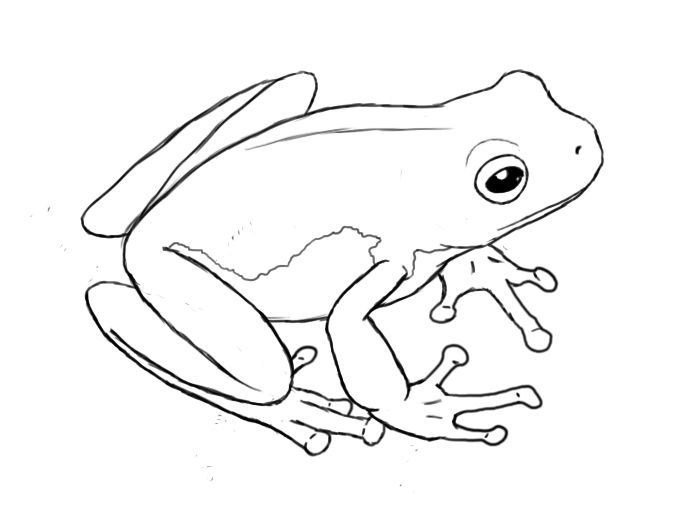
\includegraphics[width=0.4\textwidth]{dekikker}
\end{intersong}
\beginsong{De Kikker}
\beginverse
Aan den oever van de Dijle,
Diep verscholen in het riet,
Zat een kleine jonge kikker
Bij zijn moeder op de knie!
\endverse
\beginverse
"Ziet ge daar" zo sprak die moeder,
"Ziet ge daar dien ooievaar,
't Is de moord'naar van uw vader,
Hij vrat hem op met huid en haar".
\endverse
\beginverse
"Godverdomme", sprak die kleine,
"Heeft die smeerlap dat gedaan,
Als ik groot en sterk zal wezen
Zal op op zijn bakkes slaan"!
\endverse
\beginverse
Vele jaren zijn verstreken,
En de kikker leeft niet meer.
Maar de ooievaar die leeft nog,
En zijn bakkes doet nog zeer.
\endverse
\beginverse
'kHeb zoveel u nog te zeggen
Haar ge zoudt het niet verstaan
'k Zal u in uw bedje leggen..."
En daarmee is 't lied gedaan.
\endverse
\endsong